\section{Results}
\label{sec:results}

\subsection{Model Comparison}
\label{sec:res_main}
Table~\ref{tab:e1} reports the test-period accuracy of all models in the reference setting (three-year window, weekly refits). All learned models reduce the mean MAPE of the best seasonal naive benchmark (SN-DT, 4.44\%) by 33--40\%, and the ranking is remarkably stable across subsystems. The linear ARX model is the most accurate individual model, with a mean MAPE of 2.70\%, followed by the MLP (2.76\%) and the GBM (2.96\%). The simple ensemble ENS is the best model in all subsystems in terms of MAPE (2.66\% on average) and in three of the four in terms of RMSE. Errors are lowest in the North and Northeast (about 2\%) and highest in the South (about 4\%), where the load is the most temperature sensitive and where cold fronts and heat waves cause large day-to-day changes that a weather-free model cannot anticipate.

The DM tests (Table~\ref{tab:dm}) confirm that these differences are statistically significant: after the Holm correction, ARX is significantly more accurate than GBM in all four subsystems and than the MLP in three, and ENS is significantly more accurate than every individual model in at least two subsystems (than GBM and the MLP in all four). No model is significantly more accurate than ENS in any subsystem. That a regularised linear model beats a tuned gradient boosting model contrasts with the success of tree ensembles in retail and tabular competitions~\cite{makridakis2022m5,grinsztajn2022tabular}, but is consistent with the electricity price forecasting literature~\cite{lago2021benchmark}: with a strongly autoregressive target and smooth calendar effects, the 24 hour-specific linear models already capture most of the predictable structure, whereas the global tree model must learn the hour interactions from data. A hybrid in which a GBM learned the residuals of ARX was also evaluated on the validation year, but it did not improve on ARX (MAPE 2.68\% versus 2.65\%) and was discarded.

Fig.~\ref{fig:err}(a) shows that the error of every model peaks between 12:00 and 15:00 and is lowest overnight. This is the period in which behind-the-meter PV output, and thus the weather, has the largest effect on the load seen by the operator. Fig.~\ref{fig:err}(b) shows a clear seasonal pattern, with the largest errors from November to February (3.0--3.5\% averaged over subsystems), when convective rain and heat waves make both the cooling demand and the PV output volatile, and the smallest errors in July and August (about 2.1\%), during the dry austral winter; there is no upward trend over the test period.

\begin{table*}[!t]
\caption{Test-period accuracy (January 2024 -- November 2026) in the reference setting: MAPE (\%) and RMSE (MW) per subsystem, and MAPE averaged over subsystems. Best value per column in bold.}
\label{tab:e1}
\centering
\begin{tabular}{lccccccccc}
\toprule
& \multicolumn{2}{c}{North} & \multicolumn{2}{c}{Northeast} & \multicolumn{2}{c}{South} & \multicolumn{2}{c}{Southeast/C.-West} & All \\
\cmidrule(lr){2-3}\cmidrule(lr){4-5}\cmidrule(lr){6-7}\cmidrule(lr){8-9}\cmidrule(lr){10-10}
Model & MAPE & RMSE & MAPE & RMSE & MAPE & RMSE & MAPE & RMSE & MAPE \\
\midrule
\tabinput{tables/tab_e1.tex}
\bottomrule
\end{tabular}
\end{table*}

\begin{table}[!t]
\caption{Number of subsystems (out of four) in which the row model is significantly more accurate than the column model (one-sided DM test on daily MAPE, Holm-adjusted $p<0.05$).}
\label{tab:dm}
\centering
\setlength{\tabcolsep}{4pt}
\begin{tabular}{lcccccc}
\toprule
& SN7 & SNDT & ARX & GBM & MLP & ENS \\
\midrule
\tabinput{tables/tab_dm.tex}
\bottomrule
\end{tabular}
\end{table}

\begin{figure*}[!t]
\centering
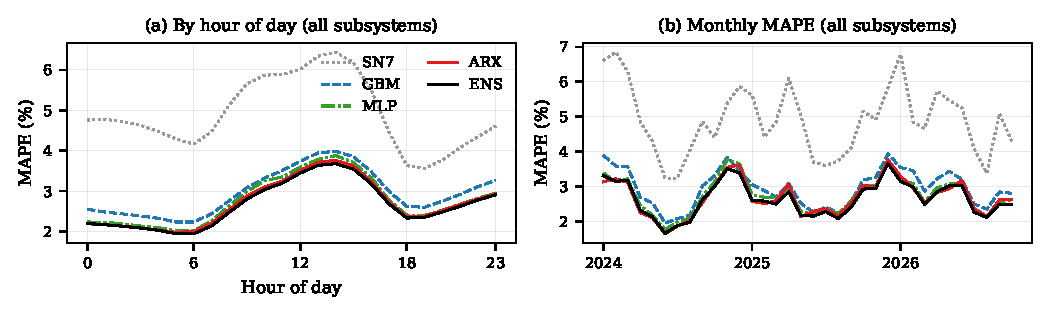
\includegraphics[width=\textwidth]{figures/fig_err_hour_month.pdf}
\caption{Test-period MAPE in the reference setting, averaged over the four subsystems: (a) by hour of the target day; (b) by month.}
\label{fig:err}
\end{figure*}

\subsection{Calibration Window and Refitting Frequency}
\label{sec:res_window}
Table~\ref{tab:e2} reports the mean MAPE of ARX and GBM for calibration windows from one year to the full history and refitting frequencies from daily to yearly. Two findings stand out. First, the refitting frequency matters much less than expected under drift: for ARX, moving from daily to yearly refits increases the MAPE by at most 0.06 percentage points (pp) for windows of two years or more, and for GBM the differences between refitting frequencies are at most 0.03~pp for every window. With level normalisation (Section~\ref{sec:method}), the slow growth of demand is absorbed by the scale $s_d$, so a model fitted a year earlier remains valid for the shape of the profile. Only ARX with a one-year window is sensitive to the refitting frequency (2.85\% with daily and 3.09\% with yearly refits), because a model fitted on a single year has seen each calendar situation only once. Second, the calibration window length matters more: one-year windows are clearly worse (ARX 2.85--3.09\%, GBM 3.23--3.25\%), and the accuracy improves up to five years for ARX (2.67\%) and up to the full history for GBM (2.83\%). Very long windows thus do not hurt, even though the load profile changed substantially over the period (Fig.~\ref{fig:profiles}): the annual Fourier terms, the lagged profiles, and the normalisation let the models represent recent profiles while benefiting from more examples of rare days, such as holidays. Averaging forecasts across windows, which is beneficial in price forecasting~\cite{hubicka2019windows,marcjasz2018windows}, brings no gain here: the average of the six weekly ARX forecasts reaches 2.67\%, equal to the best single window, and the average of the six monthly GBM forecasts 2.84\%, versus 2.83\% for the expanding window alone.

\begin{table}[!t]
\caption{Mean test MAPE (\%) over the four subsystems as a function of the calibration window and the refitting frequency (D: daily, W: weekly, M: monthly, Q: quarterly, Y: yearly). Weekly GBM refits were run only for 1- and 3-year windows. Best value per model in bold.}
\label{tab:e2}
\centering
\setlength{\tabcolsep}{2.6pt}
\begin{tabular}{lccccc|cccc}
\toprule
& \multicolumn{5}{c|}{ARX} & \multicolumn{4}{c}{GBM} \\
Window & D & W & M & Q & Y & W & M & Q & Y \\
\midrule
\tabinput{tables/tab_e2.tex}
\bottomrule
\end{tabular}
\end{table}

\subsection{Ablations}
\label{sec:res_ablation}
Table~\ref{tab:ablation} isolates the contribution of three design choices. Level normalisation is decisive for the tree model: without it, the GBM MAPE increases from 2.96\% to 3.23\%, and with an expanding window it is 3.25\% without normalisation versus 2.83\% with it (Table~\ref{tab:e2}), because the trees cannot produce values outside the range of past targets, which a growing load continuously exceeds. For ARX the normalisation is neutral (2.70\% in both cases), as expected for a linear model, and for the MLP it brings a small improvement. The special-day features reduce the MAPE of ARX by 0.24~pp and of GBM by 0.21~pp; although such days are only about 7\% of the test period, their errors are large enough to affect the overall averages (Section~\ref{sec:res_special}). The observations of the morning of day $d-1$ are the most valuable input of the tree model (without them, the GBM MAPE increases by 0.54~pp, and by 0.82~pp in the SE), and they reduce the ARX error by 0.19~pp: even 14 hours before the target day begins, the most recent load level carries information that the complete day $d-2$ does not.

\begin{table}[!t]
\caption{Ablations: mean test MAPE (\%) over the four subsystems in the reference setting.}
\label{tab:ablation}
\centering
\setlength{\tabcolsep}{3pt}
\begin{tabular}{p{0.56\columnwidth}ccc}
\toprule
Variant & ARX & GBM & MLP \\
\midrule
\tabinput{tables/tab_ablation.tex}
\bottomrule
\end{tabular}
\end{table}

\subsection{Special Days}
\label{sec:res_special}
Table~\ref{tab:daytype} breaks down the error by day type. National holidays, Carnival, Christmas and New Year's eves, and Ash Wednesday have errors 1.2--2 times those of regular weekdays for the learned models, and up to 2.3 times for the seasonal naive benchmark. Two patterns are worth noting. First, bridge days, which are not official holidays but on which many businesses close, are forecast almost as accurately as regular weekdays once they are flagged, showing that the programmatic calendar captures most of their effect. Second, different models are best on different special days, which is one reason why the ensemble is more robust than any single model; with only 3--30 occurrences of each type in the test period, however, these differences are not statistically conclusive. Days of the year-end period (December 26 to January 6), in which industrial activity is reduced, remain about 40\% harder than regular weekdays.

\begin{table}[!t]
\caption{Test MAPE (\%) by day type, averaged over the four subsystems ($n$: number of test days).}
\label{tab:daytype}
\centering
\setlength{\tabcolsep}{3pt}
\begin{tabular}{lcccccc}
\toprule
Day type & $n$ & SN7 & ARX & GBM & MLP & ENS \\
\midrule
\tabinput{tables/tab_daytype.tex}
\bottomrule
\end{tabular}
\end{table}

\subsection{Probabilistic Forecasts}
\label{sec:res_prob}
Table~\ref{tab:prob} compares the three probabilistic methods. On the validation period, the selected EQR window was $W=56$ days and the selected ACI step was $\gamma=0.005$. The quantile GBM is severely overconfident on the test period: its nominal 80\% and 90\% intervals cover only 53\% and 69\% of the observations. The quantiles are learned from in-sample fits, whose residuals are much smaller than the out-of-sample errors of a flexible model; flexible quantile regressors have no finite-sample calibration guarantee, which is precisely what motivated conformalised quantile regression~\cite{romano2019cqr}. The empirical relative-error quantiles of EQR, which are computed from genuine out-of-sample errors, are much better calibrated (77\% and 87\%) and also have a 16\% lower pinball loss than QGBM. ACI closes the remaining gap: with a small step, it attains 80.3\% and 90.1\% coverage, at the cost of intervals that are 9--15\% wider than those of EQR, and with a Winkler score very close to that of EQR.

Fig.~\ref{fig:cov} shows that the calibration of all methods varies over time. EQR coverage drops below 80\% during episodes in which the error distribution changes faster than its 56-day window can follow, mostly between September and December, when the transition from the dry winter to the hot season changes the level and the volatility of the errors, especially in the S and SE subsystems. ACI raises its intervals after such episodes and recovers the nominal coverage within a few weeks, but, because the feedback is delayed by two days and the step is small, it cannot prevent short-lived drops in coverage.

\begin{table}[!t]
\caption{Probabilistic forecasts on the test period, averaged over the four subsystems: coverage (Cov., \%), mean width (\% of mean load), and Winkler score (Wink., \% of mean load) of the central 80\% and 90\% prediction intervals, and mean pinball loss over seven quantiles (\% of mean load).}
\label{tab:prob}
\centering
\setlength{\tabcolsep}{2.8pt}
\begin{tabular}{lccccccc}
\toprule
& \multicolumn{3}{c}{80\% interval} & \multicolumn{3}{c}{90\% interval} & \\
\cmidrule(lr){2-4}\cmidrule(lr){5-7}
Method & Cov. & Width & Wink. & Cov. & Width & Wink. & Pinball \\
\midrule
\tabinput{tables/tab_prob.tex}
\bottomrule
\end{tabular}
\end{table}

\begin{figure}[!t]
\centering
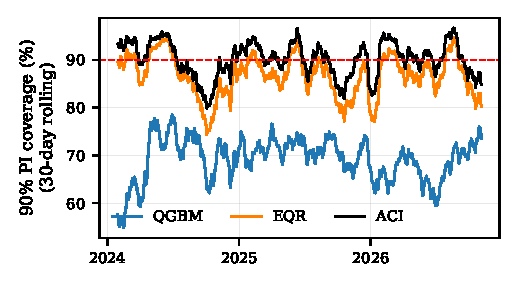
\includegraphics[width=\columnwidth]{figures/fig_coverage.pdf}
\caption{Coverage of the nominal 90\% prediction intervals over the test period (30-day rolling mean, averaged over the four subsystems).}
\label{fig:cov}
\end{figure}

\subsection{Comparison With the Official Forecast}
\label{sec:res_ons}
Table~\ref{tab:e6} compares the models fitted on the verified global load with the official ONS day-ahead forecast over the \NdaysONS{} common test days. ENS is more accurate than the official forecast in all four subsystems: its MAPE is 25\% lower in the North (1.96\% versus 2.62\%), 28\% lower in the Northeast (1.96\% versus 2.71\%), 9\% lower in the South (3.57\% versus 3.92\%), and 3\% lower in the Southeast/Center-West (2.26\% versus 2.33\%); on average, the reduction is 16\% (2.44\% versus 2.90\%). The improvement is significant according to the DM test in the North, Northeast, and South ($p<0.001$), but not in the Southeast/Center-West ($p=0.10$), where the official forecast also has a slightly lower RMSE. ARX and the MLP individually lead to the same conclusions, whereas GBM is significantly more accurate than the official forecast in the North and Northeast but significantly less accurate in the Southeast/Center-West. ENS gives the lower daily MAPE on 73\%, 70\%, 60\%, and 56\% of the days in the N, NE, S, and SE subsystems, respectively.

The error profile by hour (Fig.~\ref{fig:ons_hour}) explains these results. In the North and Northeast, the error of the official forecast rises sharply between 07:00 and 16:00, and between 10:00 and 14:00 it is 1.8 times the error of ENS in the North (4.3\% versus 2.4\%) and 1.5 times in the Northeast (3.8\% versus 2.6\%), whereas the gap is much smaller at night. In the South and Southeast/Center-West, the official forecast is slightly more accurate in the afternoon (14:00--17:00) and late evening, i.e., at the hours in which temperature drives the load, and ENS is more accurate at night and in the morning.

The midday errors of the official forecast are not random: they are a growing systematic under-forecast. Between 10:00 and 14:00, the mean relative bias of the official forecast went from $-2.8\%$, $-0.8\%$, $-0.5\%$, and $-1.0\%$ in 2024 to $-3.9\%$, $-3.0\%$, $-2.4\%$, and $-2.3\%$ in 2026 in the N, NE, S, and SE subsystems, respectively, whereas the bias of ENS stayed within $\pm1.3\%$ in every year and subsystem. Fig.~\ref{fig:ons_bias} shows the monthly midday bias together with the share of the global load supplied by MMGD: the official forecast's bias deepens as this share grows, with monthly correlations between $-0.31$ (N) and $-0.54$ (NE and S). Consistent with this, the annual MAPE of the official forecast increased from 2024 to 2026 in all subsystems (e.g., from 2.28\% to 2.83\% in the North and from 2.31\% to 2.93\% in the Northeast), whereas that of ENS remained stable (1.94\% to 1.97\% and 1.85\% to 2.04\%, respectively).

From July 2026 onwards, the midday bias of the official forecast became much smaller in all subsystems (Fig.~\ref{fig:ons_bias}), which suggests a revision of the operator's procedure. Even in these last four months (127 days), however, ENS remained significantly more accurate in the North (1.58\% versus 1.93\%), Northeast (1.77\% versus 2.24\%), and South (2.95\% versus 3.63\%), and statistically equivalent in the Southeast/Center-West (2.41\% versus 2.35\%), so the midday bias is the main, but not the only, source of the difference.

Because the exact data cut-off of the official forecast is not published, we repeated the comparison with an ARX model that does not use any observation of day $d-1$, i.e., with data only up to the end of day $d-2$. This model remains significantly more accurate than the official forecast in the North (2.07\% versus 2.62\%) and the Northeast (2.14\% versus 2.71\%), is statistically indistinguishable in the South (3.98\% versus 3.92\%), and is significantly less accurate in the Southeast/Center-West (2.54\% versus 2.33\%). The advantage in the North and Northeast therefore does not depend on the most recent observations, whereas in the two southern subsystems the information of the morning of day $d-1$ is what makes a weather-free model competitive.

Finally, the two forecasts are partly complementary. An equal-weight average of ENS and the official forecast, which requires no estimation, reduces the MAPE further in the South (3.38\%) and the Southeast/Center-West (2.07\%), the subsystems where the official forecast is competitive and presumably benefits from weather information, but not in the North and Northeast (2.11\% and 2.12\%), where the official forecast's midday bias dominates.

\begin{table*}[!t]
\caption{Comparison with the official ONS day-ahead forecast on the verified global load (common test days, January 2024 -- November 2026): MAPE (\%) and RMSE (MW). $^{+}$/$^{-}$: model significantly more/less accurate than the official forecast (one-sided DM test on daily MAPE, $p<0.05$). Best value per column in bold.}
\label{tab:e6}
\centering
\begin{tabular}{lccccccccc}
\toprule
& \multicolumn{2}{c}{North} & \multicolumn{2}{c}{Northeast} & \multicolumn{2}{c}{South} & \multicolumn{2}{c}{Southeast/C.-West} & All \\
\cmidrule(lr){2-3}\cmidrule(lr){4-5}\cmidrule(lr){6-7}\cmidrule(lr){8-9}\cmidrule(lr){10-10}
Forecast & MAPE & RMSE & MAPE & RMSE & MAPE & RMSE & MAPE & RMSE & MAPE \\
\midrule
\tabinput{tables/tab_e6.tex}
\bottomrule
\end{tabular}
\end{table*}

\begin{figure*}[!t]
\centering
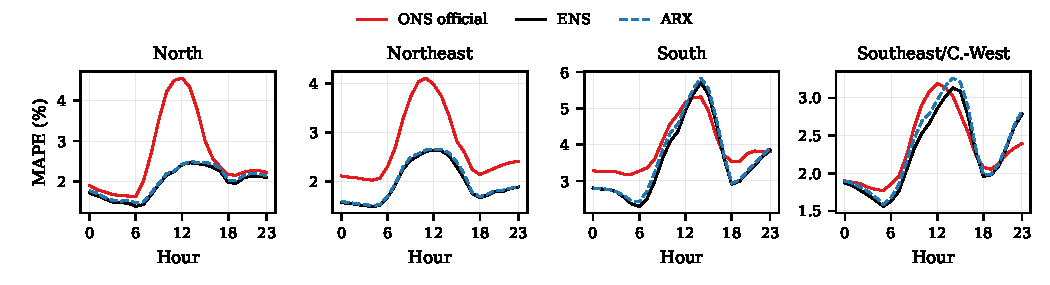
\includegraphics[width=\textwidth]{figures/fig_ons_hour.pdf}
\caption{MAPE by hour of the target day of the official ONS forecast, ENS, and ARX on the verified global load (common test days).}
\label{fig:ons_hour}
\end{figure*}

\begin{figure*}[!t]
\centering
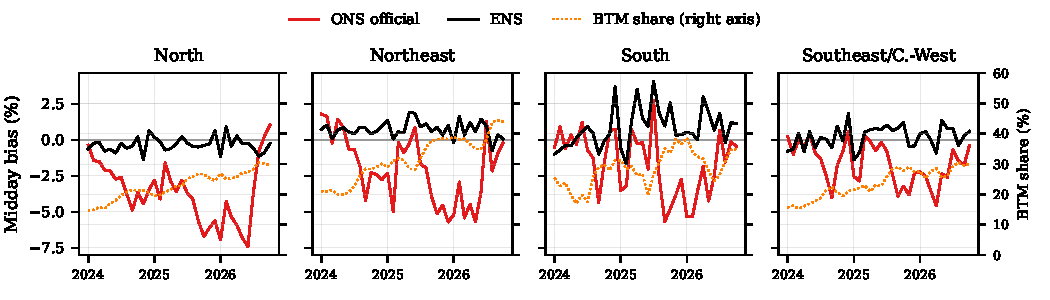
\includegraphics[width=\textwidth]{figures/fig_ons_bias.pdf}
\caption{Monthly mean relative bias (forecast minus verified, \% of verified load) between 10:00 and 14:59 of the official ONS forecast and of ENS (left axes), and share of the verified global load supplied by behind-the-meter MMGD in the same hours (dotted, right axes).}
\label{fig:ons_bias}
\end{figure*}
